%%%%%%%%%%%%%%%%%%%%%%%%%%%%%%%%%%%%%%%%%%%%%%%%%%%%%%%%%%%%%%%%%%%%%%%%%%%
%%%                                                                     %%%
%%%   LaTeX template voor het verslag van P&O: Computerwetenschappen.   %%%
%%%                                                                     %%%
%%%   Opties:                                                           %%%
%%%     tt      Tussentijdsverslag                                      %%%
%%%     eind    Eindverslag                                             %%%
%%%                                                                     %%%
%%%   7 februari 2014                                                   %%%
%%%   Versie 1.2                                                        %%%
%%%                                                                     %%%
%%%%%%%%%%%%%%%%%%%%%%%%%%%%%%%%%%%%%%%%%%%%%%%%%%%%%%%%%%%%%%%%%%%%%%%%%%%

\documentclass[eind]{penoverslag}

%%% PACKAGES %%%
\usepackage{graphicx} 		%afbeeldingen
\usepackage{algorithmic}	%algoritmes
\usepackage{amsmath}		%wiskundige notaties
\usepackage{wasysym}		%symbolen
\usepackage{float}		%zwevende objecten
\usepackage{wrapfig}		%figuren beter weergeven


\setlength\parindent{0pt}	%geen indentatie

%"Figuur" in vet
\makeatletter
\renewcommand{\fnum@figure}{\small\textbf{\figurename~\thefigure}}
\makeatother

\setcounter{tocdepth}{2}
\setcounter{secnumdepth}{2} 

\begin{document}

% == TITELPAGINA == %
\team{Indigo} % teamkleur
\members{
        Wander Bavin\\
        Vince Goossens\\
        Dimitri Jonckers\\
        Sunil Tandan\\
        Wout Vekemans} % teamleden
\maketitlepage


% == SAMENVATTING == %
\begin{abstract}
\noindent
Dit rapport documenteert onze analyse en oplossing van het volgende probleem: de constructie en operatie van een zeppelin in wedstrijdverband. Net zoals vorig semester wordt de zeppelin bestuurd door een Raspberry Pi, en heeft hij propellers om de beweging te controleren. Navigatie gebeurt op basis van een op voorhand gekend grondplan met unieke patronen van figuren dat wordt ingeladen in de software. Een algoritme gebaseerd op pattern recognition bepaalt de positie van de zeppelin. Het veld bevat tablets die QR-codes kunnen weergeven die een opdracht encoderen. De wedstrijd bestaat uit het volgen van opdrachten om naar een bepaalde positie te vliegen en uiteindelijk te landen. Beide zeppelins wisselen informatie uit met elkaar en met hun sturende pc via een server gebaseerd op RabbitMQ. Een GUI dient de toestand van het speelveld en beide zeppelins te visualiseren. Een simulator biedt de mogelijkheid om een wedstrijd na te bootsen zonder dat er echt zeppelins aanwezig moeten zijn. Al deze functionaliteiten worden ge\"{i}mplementeerd in Java.\\
\end{abstract}


% == INHOUDSOPGAVE == %
\tableofcontents\newpage


% == INLEIDING == %
\section{Inleiding}
Dit tweede deel van de bachelorproef draait nog steeds rond het aansturen van een zeppelin op basis van een Raspberry Pi. De zeppelin moet kunnen bewegen in de 3D-ruimte. Dit semester zal de zeppelin zich constant boven een speelveld bevinden waarop figuren liggen. De image recognition gebruikt de figuren om de positie exact te bepalen. De eigen zeppelin speelt een wedstrijd tegen een vijandige zeppelin van een ander team. Beide proberen ze om als eerste de opgegeven bestemmingen te bereiken en te landen op de voorziene plaats.\\
In dit document volgt eerst een korte beschrijving van het gebruikte materiaal en de fysische structuur van de zeppelin. Daarna worden de uitgevoerde testen en gebruikte algoritmes beschreven. Tot slot volgt er nog een sectie die specifiek over de gebruikte en geschreven software handelt. 

\paragraph{Fysisch ontwerp}
~\\
De zeppelin bestaat uit een houten frame waaraan 2 heliumballonnen ($\diameter$ 90 cm) vastgemaakt zijn. Aan het frame zijn een camera en een afstandssensor vastgemaakt, die beiden naar beneden gericht zijn. Zowel de camera als de afstandssensor zijn verbonden met een Raspberry Pi die in het frame zit ingebed. Het geheel bevat drie propellers: twee voor horizontale bewegingen en \'{e}\'{e}n voor verticale bewegingen.


\paragraph{Software ontwerp}
~\\
Onze software is verdeeld in twee delen. Enerzijds is er het hardware-gerelateerde deel (foto's nemen en motoren aansturen) dat op de Pi draait. Anderzijds voert de sturende pc het 'zwaardere werk' uit. (afbeeldingen verwerken,\ldots) De GUI draait uiteraard op de laptop. \\
Alle software is geschreven in Java. De communicatie tussen de zeppelins en de laptop gebeurt via een RabbitMQ server, waarlangs commando's moeten passeren die aan een vooraf afgesproken formaat voldoen. (Zie figuur \ref{schema}). \\

%% figuur van software-architectuur %%
\begin{figure}[ht!]
\centering
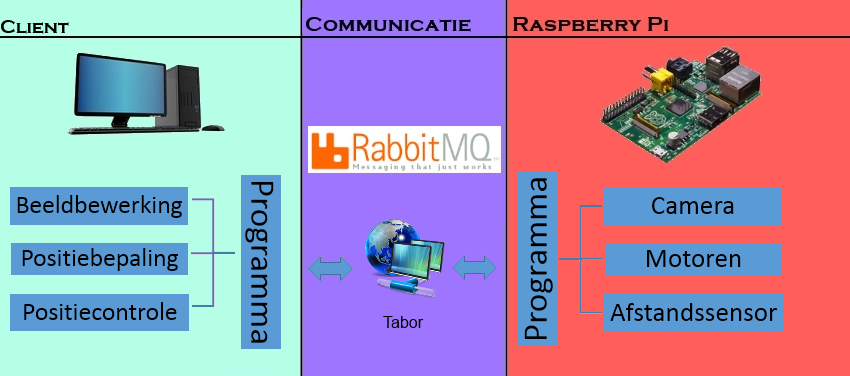
\includegraphics[height=55mm]{Schema.png}
\caption{Architectuur}
\label{schema}
\end{figure}

% == Beschrijving materiaal en bouw zeppelin == %
\section{Beschrijving materiaal en bouw zeppelin}
De basis van de zeppelin is een houten frame. Hierop zijn alle andere onderdelen bevestigd.\\
Ten eerste zijn er drie motoren vastgemaakt aan het frame. Twee van deze motoren dienen om in het horizontale vlak te bewegen. Ze zijn met haakse draairichting op het frame (zie figuur \ref{frame}) gemonteerd. Dit staat toe om een horizontale beweging te reduceren tot een beweging in x- en y-richting, zodat het niet nodig is om te draaien (tijdens het vorige semester werd al duidelijk dat dit voor sterke afwijkingen van de zeppelin zorgt). De derde propeller dient om de hoogte te regelen, en is naar beneden gericht. De propellers kunnen op volle kracht of door middel van PWM\footnote{en.wikipedia.org/wiki/Pulse-width\_modulation} worden aangestuurd (in 2 richtingen). Met deze techniek is het mogelijk om naast de richting ook de kracht van de motor in te stellen.Hardware-PWM op het motorbordje stuurt de onderste propeller aan, terwijl SoftPWM\footnote{https://github.com/Pi4J/pi4j/blob/master/pi4j-core/src/main/java/com/pi4j/wiringpi/SoftPwm.java} de horizontaal gerichte propellers regelt. 

%% figuur frame %%
\begin{figure}[h!]
\centering
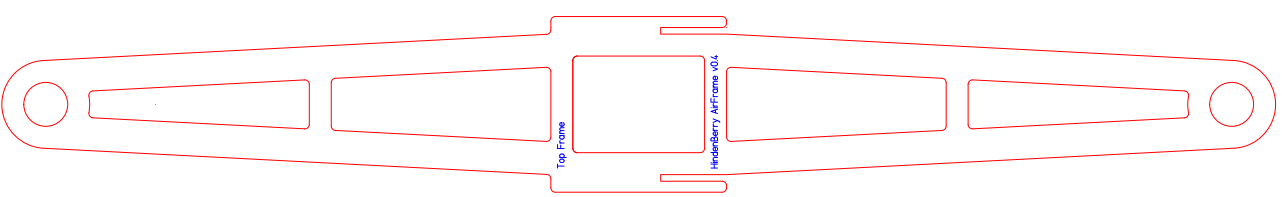
\includegraphics[scale=0.3]{upperFrame.png}
\label{frame}
\end{figure}

\begin{figure}[h!]
\centering
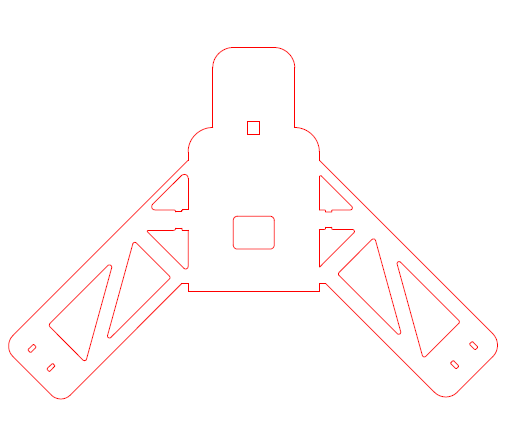
\includegraphics[scale=0.4]{lowerFrame.png}
\caption{Blueprint van het frame}
\label{frame}
\end{figure}

Er zitten ook 2 heliumballonnen ($\diameter$ 90 cm) vast aan de bovenkant van het frame. Die houden het geheel in de lucht. Ze hebben initieel een lift van 268 gr per stuk, maar dit vermindert wanneer de ballonnen doorheen de weken volume verliezen. \\

De zeppelin wordt aangestuurd door een Raspberry Pi model A. Deze heeft volgende specificaties:
\begin{itemize}
\item \emph{Processor:} 700MHz ARM
\item \emph{Geheugen:} 256MB
\item \emph{Poorten:} 1 USB 2.0, HDMI, audio out, RCA video
\item \emph{Voeding:} Micro USB
\item GPIO-pinnen om de hardware aan te sturen
\end{itemize}

In de Raspberry Pi zit een SD-kaart van 4 GB. Hierop staat Raspbian, het standaard besturingssysteem van de Raspberry Pi. Er is nog voldoende ruimte over om onze eigen programma's als jar-file op de Pi te zetten. \\

Verder mnaakt de zeppelin gebruik van nog twee apparaten:
\begin{itemize}
\item \textbf{De camera} laat toe foto's te nemen met een maximum resolutie van 5 MP. Hij wordt in deze opdracht vooral gebruikt voor het bepalen van de positie van de zeppelin. Hiervoor neemt hij foto's van de patronen op de grond die vergeleken worden met het gekende grondplan. Daarnaast kan de camera video's maken met resoluties tot 1080p.

\item \textbf{De afstandssensor} meet met behulp van ultrasone trillingen de afstand tussen de zeppelin en de grond of muur. In ons project stuurt hij het hoogteregelend PID-algoritme aan. 
\end{itemize}

%% foto volledig frame
\begin{figure}[ht!]
\centering
\includegraphics[height=60mm]{FullFrame.jpg}
\caption{Frame met gemonteerde onderdelen}
\label{zeppFrame}
\end{figure}

Het geheel is gemonteerd met plakband en zipties. Bekertjes onderaan de zeppelin dragen de ballast, zo bepaald dat de zeppelin lichtjes zakt als de motoren afstaan. Zout dient als gewicht, zodat het mogelijk is om nauwkeurig het gewicht te regelen. Tijdens het landen steunt het geheel op twee pootjes, gemaakt van piepschuimen bekertjes. \\

Voor de finale demo hebben we een nieuw frame ontwikkeld. De motoren staan nu haaks op elkaar wat voor een symmetrische gewichtsverdeling zorgt. De pootjes en ballast blijven behouden. Omwille van geometrische redenen (ori\"entatie van de zeppelin in xy-vlak) is de camera in het nieuwe frame 45 graden gedraaid. \\

% == Testen == %
\section{Testen}

Om er zeker van te kunnen zijn dat het aansturen van de zeppelin correct gebeurt, is het nodig dat de componenten getest worden. In deze sectie volgt hierover meer informatie.

\subsection{Afstandssensor}
Voor gedetailleerde gegevens verwijzen we naar het verslag over onze zeppelin van het eerste semester (versie 2). Hier merken we dat een enkele waarde van de sensor niet noodzakelijk de correcte afstand weergeeft. Daarom houdt de afstandssensor de laatste 10 gemeten waardes bij. De huidige hoogte wordt gegeven als de mediaan van deze waarden (rolling median techniek). Door het gebruik van deze techniek hebben uitschieters en foute meetwaarden minder invloed op het eindresultaat. Het interval tussen twee metingen hebben we kunnen terugbrengen tot 20 ms.\\

\subsection{Camera en pattern recognition}
Om de implementatie van pattern recognition te kunnen optimaliseren, hebben we verschillende nieuwe testen moeten doen met de camera. De tests proberen de verschillende moeilijkheden van de real time uitvoering te simuleren. De factoren die de positiebepaling aan de hand van de pattern recognition be\"invloeden, hebben vooral betrekking tot de lichtintensiteit, de hoogte en het nemen van foto’s terwijl de zeppelin beweegt. De verschillende factoren en hun bijbehorende tests worden hieronder besproken.

\subsubsection{Lichtintensiteit}
De intensiteit van het licht be\"{i}nvloedt de detectie van de contouren en vooral het correct herkennen van kleuren. We hebben geprobeerd om vormen en kleuren te herkennen in een kamer met kunstlicht en een kamer met natuurlijk licht. In beide situaties konden de kleuren herkend worden, mits het correct afstellen van de grenzen voor bepaalde kleuren. Als dat calibratieproces op een nauwkeurige manier kan gebeuren voor de demo zullen alle kleuren herkend worden.

\subsubsection{Hoogte}
De hoogte van de zeppelin tijdens de fotoregistratie heeft gevolgen voor het aantal vormen die geregistreerd worden en de afstand tussen de vormen op de foto. Er is een minimaal aantal vormen nodig om de positie te bepalen (3 figuren). Een succesvolle verwerking vereist een minimale hoogte, die we zullen bepalen door verschillende hoogtes te testen. Te weinig vormen op de foto zorgen ervoor dat de positie niet bepaald kan worden. Het aantal pixels tussen de verschillende contouren kan ook een negatief effect hebben op de differentiatie van de verschillende vormen. De camera neemt foto’s van een patroon van vormen gepositioneerd onder de zeppelin waarbij de hoogte steeds varieert.\\
%TODO MSS EFFECTIEF TESTEN? OF IETS VERZINNEN. BIJ BEWEGING OOK. !!
\subsubsection{Beweging}
Er is een bepaalde verwerkingstijd nodig om de genomen foto's om te zetten naar co\"ordinaten. Daarom moet ervoor gezorgd worden dat de zeppelin niet te snel beweegt. Anders is het mogelijk dat de positie van de zeppelin op het moment dat hij co\"ordinaten doorkrijgt, zeer hard afwijkt van waar hij denkt te zijn. Verder wordt het moeilijk om de contouren te herkennen als de zeppelin aan te hoge snelheid vliegt. De foto's worden dan te wazig om te herkennen.

\subsubsection{Kleurherkenning}
Voor het bepalen van de kleur van een herkende figuur is er eerst getest met RGB-waarden. Dit gaf oorzaak aan een aantal onverklaarbare foutmeldingen, waardoor er is overgeschakeld op HSV. Dit werkt nu zeer goed: voor elke kleur kan een specifiek gebied worden afgebakend. 

\subsubsection{Vormherkenning}
Voor het herkennen van vormen zijn er verschillende methodes geprobeerd. Een eerste plan was om met convex omhullende figuren te werken en dan de oppervlakteverhouding te bepalen tussen contour en omhullende. Dit had weinig zinvol resultaat omdat deze waarden heel dicht bij elkaar liggen. Een andere aanpak was controleren of een figuur al dan niet convex is (onderscheid tussen hart/ster en cirkel/rechthoek), maar dit reageerde niet zoals verwacht. Ook is er geprobeerd om met de pixeloppervlakte van de benaderde contour te bepalen welke vorm het was. Elke vorm heeft een karakteristieke oppervlakte, maar deze pixeloppervlakte is afhankelijk van de hoogte en een eenduidig verband tussen de pixeloppervlakte en de hoogte kon niet gevonden worden. \\
Voor de rechthoek is er geprobeerd om te controleren of er twee evenwijdige lijnen waren. Dit bleek door onnauwkeurigheden bij het omzetten naar contouren onbetrouwbaar te zijn. Een andere methode benaderde telkens de hoek tussen opeenvolgende punten van de rechthoek. De hoek zou meestal 180 graden zijn. De verhouding van het aantal hoeken ongeveer gelijk aan 180 graden op het totaal aantal hoeken geeft dan een uitsluitingsmethode voor de rechthoek. Voor het hart is deze verhouding echter vaak ongeveer hetzelfde. \\
Om een cirkel te detecteren is er gewerkt met de oppervlakte van de berekende binnen- en buitencontour. Door de fout op de gemiddelde oppervlakte van die twee contouren te vergelijken met de effectieve oppervlakte zou een cirkel kunnen worden herkend, maar dat kon ook geen uitsluiting geven tussen andere figuren. \\
Voor het herkennen van een ster zijn er al een aantal verschillende methodes geprobeerd. E\'en van de methodes gaat uit van de vijf buitenste hoekpunten (de punten die het verst van het middelpunt liggen). Al deze buitenste hoekpunten zouden op een hoek $2\pi/5$ van elkaar moeten liggen. Dit is vaak niet correct, omdat het middelpunt van de figuur lang niet altijd exact kan bepaald worden en over het algemeen de contourpunten van de ster slecht benaderd worden. Een andere mogelijkheid is het berekenen van de verhouding tussen het buitenste hoekpunt en het binnenste hoekpunt (deze verhouding geldt altijd, omdat ze hoogte onafhankelijk is), maar ook dit is om dezelfde reden geen goede methode.\\
Uiteindelijk is er voor elk van de vier vormen een methode gevonden die vrij nauwkeurig bepaalt of een bepaalde contour al dan niet een hart, ster, \ldots is. Voor de uiteindelijk gebruikte methodes verwijzen we u door naar de sectie over algoritmes.

\subsection{Motoren}
In het eerste semester hebben we uitgebreide testen gedaan over de mogelijkheden van PWM. Het werd duidelijk dat het nodig ging zijn om constant de hoogte te controleren en bij te sturen. Daarnaast bleek het ook moeilijk om horizontale bewegingen exact uit te voeren omdat de zeppelin zeer gevoelig is voor allerlei veranderingen van de windomstandigheden in de omgeving: een andere zeppelin die beweegt, de airco, \ldots \\

In het tweede semester hebben we enkele testen opnieuw moeten uitvoeren, voornamelijk gelinkt aan het gebruik van SoftPWM. We hebben gekeken hoe het zit met de minimum waarde waarbij het vermogen groot genoeg is om voor beweging te zorgen (deze blijkt niet aanwezig bij software-PWM: zelfs 1/100 zorgt voor beweging, bij hardware-pwm is er wel een minimumwaarde). Bij dit testen hoort ook het tunen van PID-waardes voor alle motoren, omdat niet elke motor exact even sterk is. \\

% == ALGORITMES == %s
\section{Algoritmes}
\subsection{Verticale bewegingen}
Om naar een bepaalde hoogte te stijgen, maken we gebruik van een PID-algoritme\footnote{http://www.csimn.com/CSI\_pages/PIDforDummies.html}. Hierbij gaan we op basis van de huidige fout in hoogte, bepalen of de zeppelin moet stijgen of dalen en met welke kracht. Daarnaast wordt rekening gehouden met de afgeleide, om toekomstige veranderingen te voorspellen. Tenslotte is er de integraal, die fouten uit het verleden voorstelt. Op basis hiervan wordt een pwm-waarde voor de motor gegeven. Het algoritme wordt aangepast aan het gewicht van onze zeppelin en de kracht van de gegeven motoren. \\
De output wordt berekend op basis van deze formule:

\begin{equation}
 output = Kp*error + Ki*integral + Kd*derivative
 \label{PID}
\end{equation}

Hierin zijn Kp, Ki en Kd constanten die we hebben moeten bepalen. Eerst hadden we enkel rekening gehouden met de huidige error (Ki = Kd = 0), maar dit bleek er voor te zorgen dat de zeppelin veel te snel naar een bepaalde hoogte gaat en er dan ver boven of onder gaat. We hebben dit opgelost door Kd te verhogen. Door deze groot te maken, gaat de zeppelin veel rustiger naar de opgegeven hoogte en gaat hij er niet voorbij.In het tweede semester tuneden we de waarden van deze constanten opnieuw, aangezien er nieuwe volle ballonnen gegeven waren en we een ander frame gebruiken. \\

Er is een HeightController die vergelijking \eqref{PID} implementeert, en die er voor gaat zorgen dat de zeppelin zijn hoogte behoudt of naar een gevraagde hoogte gaat. Deze gaat om de 0.1 s de hoogte controleren en de PWM-waarde bijsturen. \\



\subsection{Pattern recognition}
De camera neemt foto’s van de patronen op het veld onder de zeppelin. De Raspberry Pi bewerkt deze foto’s met behulp van zelfgeschreven software. Op elk geregistreerd beeld wordt dezelfde sequentie van operaties uitgevoerd. \\

Als eerste gaat de software een kleurfiltratie toepassen op de foto. Dit gebeurt door de foto naar een HSV-digitale voorstelling te converteren. De minimale en maximale waarden voor respectievelijk H,S en V, die karakteristiek zijn voor de mogelijke kleuren, bepalen de aanwezige kleur. Hierdoor bekomt men voor elke kleur een binaire foto waarop alleen de geslecteerde kleur zichtbaar is. Enkel de kleuren uit de opgave blijven hierdoor over. Daarna worden de vijf binary foto's samengevoegd in \'e\'en foto. Voor een visualisering van dit proces, zie figuur \ref{imageReco}.\\
De vormherkenningalgoritmes (pattern recognition) registreren de contouren van de vormen uit deze samengevoegde afbeelding en halen de nuttige contouren uit het waargenomen beeld. Operaties in het algoritme verwijderen contouren die geen betrekking op de vormen.\\

\begin{figure}[H]
\begin{center}
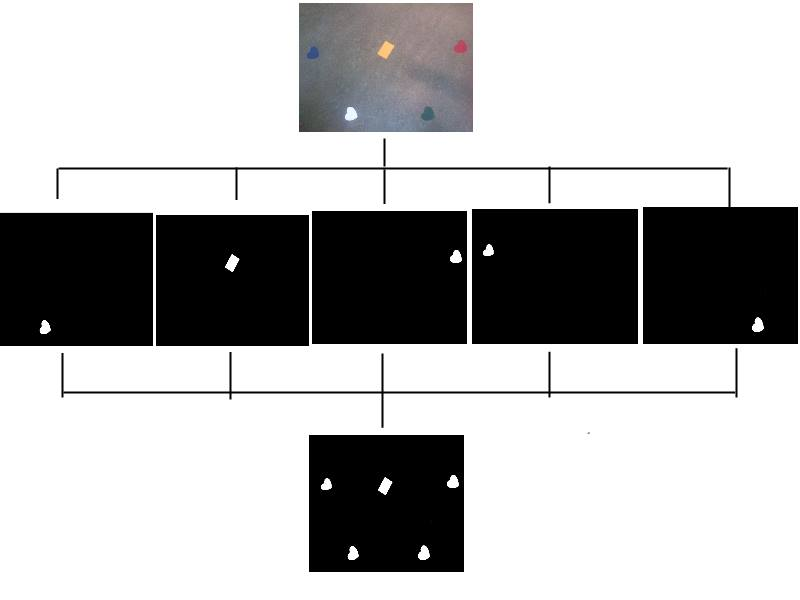
\includegraphics[width=0.8\textwidth]{imagerecognition.jpg}
\end{center}
\caption{Visualisering van kleurfiltratie}
\label{imageReco}
\end{figure}

De herkenning van vormen gebeurt op basis van de eigenschappen van de vormen. Deze eigenschappen hangen af van de oppervlaktes.
Om een rechthoek te onderscheiden van andere vormen berekent een methode van opencv de omhullende rechthoek. De verhouding van de oppervlakte van deze verkregen rechthoek en de oppervlakte van de gevonden contour is ongeveer gelijk aan 1. Dit geldt alleen voor een rechthoek. \\
Gelijkaardig om een cirkel te onderscheiden berekent een andere methode een omhullende cirkel. De verhouding van de oppervlakte van de bounding circle en de oppervlakte van de contour zelf is ongeveer gelijk aan 1.\\
Om een ster te herkennen wordt er gebruikt gemaakt van een convexe omhullende contour. De verhouding van de oppervlakte van deze convexe omhullende en de contour is ongeveer gelijk aan 1,5. Om de verschillende vormen beter te onderscheiden worden bij alle symbolen de oppervlakte van hun contouren vergeleken met de bounding rectangle, bounding circle en convex hull. Voor gedetailleerde cijfers, zie tabel \ref{recognitionTable}.\\


\begin{table}[h]
\begin{center}
\begin{tabular}{r|c|c|c}

Vorm		&	omhullende rechthoek	&	convex omhullende	&	omhullende cirkel\\
\hline
						
Rechthoek	&	\textless1,1		&	\textless1.05		&	1,5-1,9\\
Cirkel		&	1,2-1,3			&	\textless1.05		&	\textless1,3\\
Hart		&	1,2-1,4			&	\textless1.05		&	1,4-1,6\\
Ster		&	\textgreater1,9		&	\textgreater1.4		&	\textgreater1.9\\

\end{tabular}
\caption{Verhoudingen van contour en een aantal omhullende figuren}
\label{recognitionTable}

\end{center}
\end{table}


Hierdoor vinden we de symbolen die aanwezig zijn op deze afbeelding. De symbolStabilizer zorgt voor een extra foutreductie door te verifieren of een gevonden symbool op een bepaalde positie kan staan. Bijvoorbeeld als er bij voorgaande twee afbeeldingen een ster wordt herkend op een bepaalde positie en dit keer een rechthoek herkend wordt zal symbol stabalizer toch een ster terug geven. \\ 

Na de herkenning van de bymbolen probeert de software een gelijkzijdige driehoek te bepalen. Indien er minder dan drie symbolen volledig herkend worden, maar van een andere figuur toch de kleur is bepaald, zal er indien mogelijk toch een gelijkzijdige driehoek gevormd worden. Als er meerdere driehoeken gevonden worden, selecteert het algoritme diegenen die het dichtste bij het middelpunt van de foto staat.\\


\subsection{Locatiebepaling}
Om de locatie te bepalen wordt er gebruik gemaakt van een set van symbolen. Deze zijn in het ideale geval herkend door het pattern recognition algorithm. Elk symbool heeft een kleur en vorm en een x- en y-coördinaat binnen de afbeelding. Een driehoek symbolen bepaalt eenduidig de locatie van de zeppelin omdat elke driehoek maar \'e\'en keer mag voorkomen.

Een eerste mogelijkheid (de eenvoudigste) is dat het er reeds een driehoek van symbolen werd gevonden. De image processing heeft al bepaald welk van deze drie punten het dichtst ligt bij het middelpunt. Nu worden de overige twee punten gesorteerd op poolco\"ordinaat. Dan kan het matchen met het veld beginnen (zie verder). \\

Een andere mogelijkheid is dat er geen driehoek werd gevonden, maar wel een aantal symbolen. Eerst bepaalt het algoritme (voor pseudocode: zie verder) welk van de gegeven symbolen het meest centraal ligt ten opzichte van de andere symbolen. Dit symbool wordt het middelpunt. Vervolgens zoekt het algoritme driehoeken. Een driehoek bestaat uit het middelpunt en twee punten die op de kortst mogelijke afstand van elkaar liggen. Hiervoor kijken we welke punt er het dichtst bij het middelpunt ligt, en filteren we de andere punten zodat we enkel punten overhouden waarvoor de afstand tot het middelpunt binnen een bepaalde marge ligt (1.2x kortste afstand). Deze punten worden gesorteerd op poolco\"ordinaten. Vervolgens nemen we de punten per twee samen met het middelpunt. Deze twee punten mogen wel maximum 1,2x de kortste afstand uit elkaar liggen (voor het geval er symbolen ontbreken) en het tweede punt moet in wijzerzin van het eerste punt liggen. \\

In elk van beide gevallen hebben we nu een driehoek of meerdere driehoeken. Dan kan het echte vergelijken met het raster gebeuren: alle punten van het veld worden afgegaan. Indien het middelpunt overeen komt met een punt uit het raster, worden alle buren van dit punt opgevraagd. Indien de andere twee punten van de gevonden overeen komen met twee buren, die ook naast elkaar liggen en in dezelfde volgorde staan, hebben we een match en hebben we de locatie gevonden. De locatie die wordt teruggegeven is de locatie van het middelpunt.\\

Opdat een symbool overeenkomt met een symbool uit het veld, moeten ze dezelfde kleur en vorm hebben. Echter ook wanneer de vorm niet herkend is ('unrecognised') wordt dit als een match gerekend. Dit kan bijvoorbeeld het geval zijn indien een onvolledige figuur aan de rand van de afbeelding werd genomen om een driehoek te vormen, zodat enkel de kleur bekend is. \\

\textbf{Locate (No triangle): }
\begin{algorithmic}

	\STATE in: Symbols; out: location
	\STATE Symbol center = calculateCenter(symbols)
	\STATE Symbol closestToMid = closestSymbol(symbols,center)     //get symbol closest to center symbol
	\STATE closestToMidDist = dist(center,closestToMid)
	\STATE List \textless Symbol\textgreater neighbours = filter(symbols,1.2*closestToMidDist)
	\STATE neighbours = sortPolar(neighbours,center)     //sort around center
	\FOR {Symbol s1 in neighbours}
		\STATE s2 = next(s1) //symbol following s1
		\IF{dist(s1,s2) $\le$ 1.2*closestToMidDist \&\& clockwise(s1,s2)}
			\STATE location = match(center,s1,s2)
		\ENDIF
	\ENDFOR
	
\end{algorithmic}
~\\
\textbf{Match:}
\begin{algorithmic}
\STATE In: center, s1, s2; out: location
	\FOR{Symbol s on map}
		\IF{s matches center}
			\FOR{Symbol sm1 in map.neighbours(center)} 
				\STATE sm2 = next(sm1)
				\IF{s1 matches sm1 \&\& s2 matches sm2}
					\STATE location found
					\STATE return center.coordinates
				\ENDIF
			\ENDFOR
		\ENDIF
	\ENDFOR
\end{algorithmic}

Het algoritme bepaalt vervolgens de hoek. De locatie geeft de positie van de drie gevonden figuren weer. Twee van deze fiugren liggen horizontaal op het raster. De rotatiehoek van de lijn waarop deze twee figuren liggen op de foto ten opzichte van de horizontale lijn op het raster wordt bepaald aan de hand van wiskundige berekeningen (verschil tussen x- en y-co\"ordinaat in de afbeelding en de tangens).\\

Hiervoor wordt een onderscheid gemaakt op basis van de groottes van de co\"ordinaten (x1 \textless  x2?, y1 \textless  y2?), om aan de hand daarvan een bepaalde transformatie te doen op de hoek gevonden van de tangens (omdat de positiecontroller de hoek in een bepaald formaat verwacht en om alle hoeken tussen $–\pi$ en $\pi$ te vinden). Voor dit algoritme geven we geen pseudocode, aangezien het grotendeels uit een aantal if-tests bestaat. Door de manier van werken is deze hoek volledig nauwkeurig. \\

Nu zijn er dus \'e\'en of meerdere mogelijke posities en hoeken bepaald. Indien er meerdere zijn bepaald (bijvoorbeeld doordat een vorm niet herkend was waardoor deze driehoek met meerdere driehoeken overeenkomt of doordat meerdere driehoeken uit een set van symbolen werden gehaald), kiest het algoritme degene het dichtst bij de vorige positie.

\subsection{Horizontale bewegingen}
Voor bewegingen in het horizontale vlak maken we eveneens gebruik van PID-gebaseerde algoritmes. We gebruiken twee afzonderlijke algoritmes die tegelijk lopen (voor de x- en y-richting). De locatiebepaling bepaalt voor elke nieuwe foto de positie binnen en de draaiing ten opzichte van het veld. De af te leggen afstand wordt ontbonden twee loodrechte bewegingen(x en y ten opzichte van het veld). De zeppelin bevindt zich in het middelpunt van het nieuwe co\"ordinatenstelsel. De co\"{o}rdinaten van de bestemming in het geroteerde en verschoven assenstelsel bepalen dus exact hoeveel we in x- en y-richting (tov zeppelin) moeten bewegen. De omzetting gebeurt in 2 stappen, met eerst een verschuiving:
\begin{equation}
 \begin{cases}
  x_{shifted} = x_{destination} – x_{zeppelin}\\
  y_{shifted} = y_{destination} – y_{zeppelin}
 \end{cases}
\end{equation}



Hierna vindt een rotatie plaats volgens de hoek $\alpha$ waaronder de zeppelin gedraaid staat ten opzichte van het rooster (rekening houdend met de richting van het frame):
\begin{equation}
 \begin{cases}
 x_{new} = x_{shifted}*cos(\alpha) + y_{shifted}*sin(\alpha)\\
y_{new} = -x_{shifted}*sin(\alpha) + y_{shifted}*cos(\alpha)
 \end{cases}
\end{equation}

Nu geven we deze nieuwe x- en y-waarden als bestemming door aan de bijbehorende PositionController, zodat de PID-regelaar de juiste motor bijstuurt. Zie verder voor het UML-schema met de klassen die de horizontale navigatie gebruikt. (figuur \ref{navigation}).

% == SOFTWARE == %
\section{Software}

Alle software voor dit project is in Java geschreven. Deze keuze is in het eerste semester al gemaakt omdat dit voor het hele team de meest gebruikte programmeertaal was en omdat er voldoende voorbeeldcode te vinden was om te programmeren op de Pi. We hebben in het eerste semester ook geen problemen gehad met het implementeren van functionaliteit in Java (aansturen motoren, QR-codes). \\
Een andere oplossing, door veel concurrenten gekozen, is Python. Een nadeel hiervan is dat iedereen dan een nieuwe taal zou moeten leren, wat het ontwerpproces enorm vertraagt. Voor Python is wel meer voorbeeldcode te vinden voor de Raspberry Pi. Om de redenen hierboven beschreven hebben we echter voor Java gekozen. Dit semester zijn we wel op veel moeilijkheden gestoten bij het implementeren van image recognition in Java.

Een gedeelte van de code is overgenomen van ons project van vorig semester. Deze is echter volledig opgefrist, waardoor de code veel overzichtelijker is geworden. Stukken software die toen door tijdsgebrek zomaar ergens werden bijgezet, zijn verplaatst naar waar ze echt thuishoren. Enkele basiselementen zoals het aansturen van de motoren blijven echter hetzelfde.

\subsection{GUI}
De GUI stelt de gebruiker in staat om vanaf een pc verbinding te maken met de RabbitMQ-server die het speelveld en de zeppelins controleert. De GUI geeft dan informatie weer over het speelveld, de co\"{o}rdinaten van de zeppelins en de bestemming. \\

%TODO AFBEELDING VAN DE GUI 
%GUI afbeelding %
\begin{figure}[H]
\begin{center}
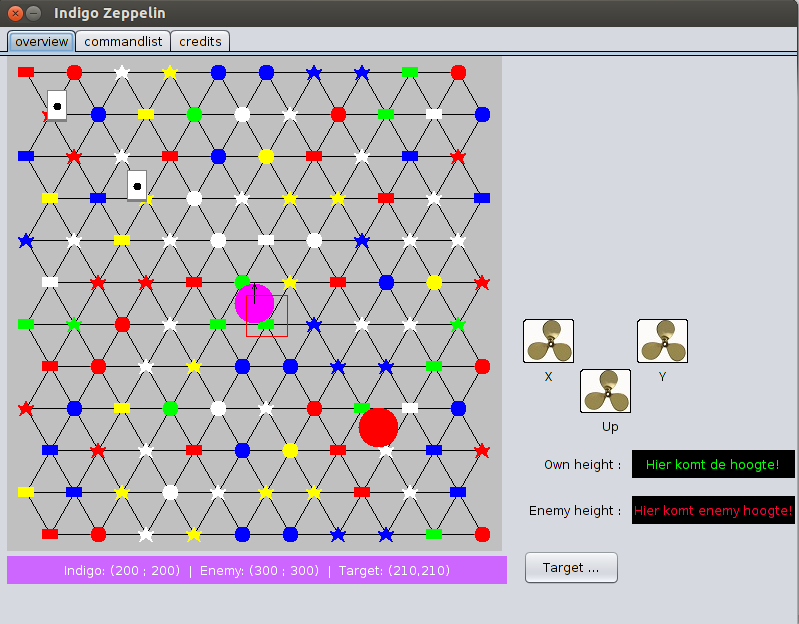
\includegraphics[width=0.6\textwidth]{GUI.png}
\end{center}
\caption{GUI}
\label{GUI}
\end{figure}

De eerste tab (`overview') toont de hoogte van beide zeppelins, alsook de toestand van de eigen propellers. Een kaart geeft de locaties van de zeppelins weer. De kaart wordt ingelezen en omgezet naar een afbeelding. Op de afbeelding verschijnen ook de posities van de eigen zeppelin en de vijandige zeppelin, en de bestemming. Naast de kaart toont de GUI de hoogte van de zeppelins en staat er een overzicht van de laatste berichten die zijn uitgewisseld tussen de pc en de zeppelin. Er is ook ruimte voorzien om de meest recent herkende afbeelding weer te geven op het scherm. \\

De tweede tab geeft een uitgebreider overzicht van alle informatie die wordt uitgewisseld tussen server, GUI en zeppelin, met een tijdsindicatie. Er is de mogelijkheid om berichten te filteren op type. \\

De derde tab ('credits') geeft wat versie-informatie en auteursrechterlijke informatie over het programma.

\subsection{Client pc: pattern recognition, locatiebepaling en horizontale beweging}
 Oorspronkelijk was het plan om het grootste deel van de programma's (waaronder image regcognition) op de Pi te laten draaien. We ondervonden echter veel problemen om openCV werkend te krijgen op de Pi en belsoten om image recognition op de client pc uit te voeren. In dit geval is het ook logisch de locatiebepaling en locatiecontrole op deze pc te zetten, aangezien dit de volgende stappen zijn nadat de figuren herkend zijn. Dit zorgt ervoor dat enkel de locatie moet worden doorgestuurd en niet de afbeelding.\\

De zeppelin biedt via een webserver afbeeldingen aan (zie verder).De slient vraagt om de 0.5 s de recentste afbeelding. Deze wordt dan omgezet naar een lijst van figuren door de ImageProcessor. Deze pattern recognition is gemaakt met behulp van de Java-library OpenCV\footnote{http://opencv.org/}. Hiermee kan detectie van vormen en kleuren worden ge\"{i}mplementeerd. De LocationLocator bepaalt hieruit de huidige postie van de zeppelin. Hierna bepaalt de positionController de af te leggen afstand in x en y. Beide richtingen hebben een PositionController, die met een PID-algoritme de pwm-waarde bepaalt. Deze worden als low-level commands naar de zeppelin gestuurd.\\

De client bevat naast de hierboven beschreven software ook de GUI. Een controlerende klasse stuurt relevante informatie door naar de GUI. Daarnaast kijkt hij of de zeppelin zich bij een tablet waar hij naartoe moet bevindt (want dan moet deze worden gevraagd de QR-code te tonen en moet uit de afbeelding een opdracht worden gelezen) en of de zeppelin bij de bestemming is (want dan moet er worden geland).\\

%Klassendiagram Bewegingen
\begin{figure}[H]
\begin{center}
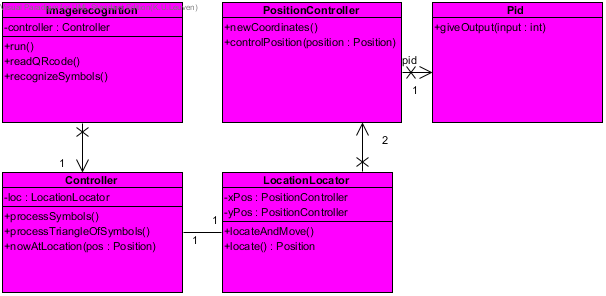
\includegraphics[width=\textwidth]{classdiagrampeno.png}
\end{center}
\caption{UML-schema horizontale bewegingen}
\label{navigation}
\end{figure}

\subsection{Connectie}
De verbinding tussen Pi en laptop is volledig veranderd ten opzichte van het eerste semester. Voordien wisselden sockets informatie uit, op een virtueel netwerk gehost vanuit een laptop. Communicatie verliep via sockets over dit netwerk. De Pi was de server omdat deze de sockets initialiseerde.\\
Deze opdracht verplicht ons een RabbitMQ-server\footnote{www.rabbitmq.com} te gebruiken. Voor de eerste tussentijdse demo startte de server op een eigen laptop. Voor de tweede demo is een server voorzien. We hebben nu dus de server (de exchange) die losstaat van de rest van het programma en de twee clients: de zeppelin (Pi) en de client-pc. Zowel pc als Pi connecteren dan op een exchange genaamd ‘server’. Elke boodschap die wordt uitgewisseld krijgt een bepaalde sleutel toegewezen, die de inhoud en de bestemming aangeeft. Een boodschap wordt dan naar de exchange verstuurd. De exchange weet dankzij de sleutel naar welke queue hij de boodschappen moet versturen. Zowel de client als de Pi abonneren zich op queues met een bepaalde sleutel, afhangende van welke gesleutelde boodschappen ze willen ontvangen. Om gebruik te maken van RabbitMQ in onze code moesten er enkele libraries\footnote{http://www.rabbitmq.com/java-client.html} toegevoegd worden. \\

Over de RabbitMQ server kunnen naar de zeppelin high-level en low-level commands worden gestuurd. High-level commands zeggen bijvoorbeeld dat de zeppelin naar een bepaalde plaats moet gaan, terwijl low-level commands naar een specifieke motor een pwm-waarde sturen. Aangezien bij ons de client de navigatie regelt, zijn de high-level commando's voor locatie enkel belangrijk voor de client die de zeppelin aanstuurt. Low-level commands daarentegen zijn relevant voor de zeppelin, alsook high-level commando's voor hoogte (bijvoorbeeld om te landen). \\


Op het sequentiediagram (zie figuur \ref{Sequence}) is te zien hoe de client een low-level commando voor het aanschakelen van de motoren aan een bepaalde snelheid doorgeeft naar de Pi. De PositionController stuurt een commando naar de zeppelin. Klasses voor communicatie versturen en ontvangen de boodschap (met toevoeging van correcte sleutel) via RabbitMQ. De Main-klasse op de zeppelin geeft het commande door aan de MotorController. Die zal uiteindelijk bepalen dat de x-motor aan een bepaalde SoftPwm-value moet draaien.
\\

%Sequentiediagram communication Pi Client
\begin{figure}[H]
\begin{center}
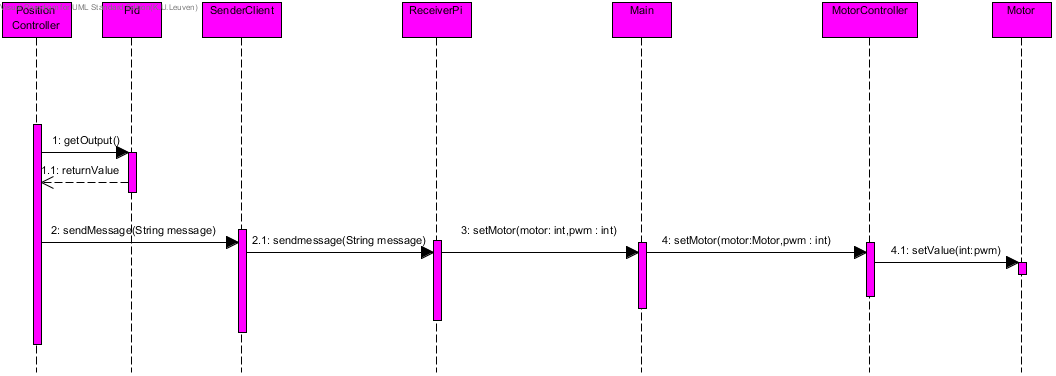
\includegraphics[width=1\textwidth]{SequenceDiagram1.png}
\end{center}
\caption{Sequentiediagram van de communicatie}
\label{Sequence}
\end{figure} 

\subsection{Zeppelin}
Er is nog maar een klein deel van de software dat draait op de zeppelin (Pi). Het belangrijkste deel hiervan is de motorcontroller, die de motoren aanstuurt op basis van low-level commando's. Die commando's komen van de client, in combinatie met gegevens van de hoogtecontroller die ook op de Pi draait. Verder is er een thread die constant de hoogte meet en een thread die afbeeldingen neemt met de camera en deze opslaat. Voor een overzicht van de klassen die op de Pi draaien, zie figuur \ref{softwareZeppelin}.\\

De Pi slaat de gemaakte afbeeldingen op in het gehuegen. Dezen kunnen dan via een webserver opgehaald worden. De reden dat dit via een webserver gebeurd, is om snelheidsredenen. Op deze manier kan een afbeelding worden doorgestuurd in minder dan 0.1 s. We hebben geprobeerd dit te doen via de RabbitMQ server, maar dit zorgde voor een te grote vertraging (ongeveer 7 s, zelfs op een lage resolutie). \\

\begin{figure}[H]
\begin{center}
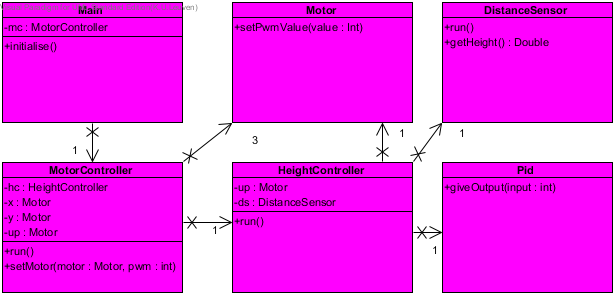
\includegraphics[width=\textwidth]{classdiagrampeno2.png}
\end{center}
\caption{UML-schema software zeppelin}
\label{softwareZeppelin}
\end{figure}

\subsection{Simulator}
Er is een simulator beschikbaar, die de toestand van het spel simuleert. Dit stelt ons in staat om algoritmes (bijvoorbeeld om een tegenstander te ontwijken) uit te testen zonder dat we echt met twee zeppelins op het speelveld moeten zitten.\\
In principe wordt gebruik gemaakt van 2 simulators: eentje voor de eigen zeppelin en eentje voor de vijand. De eerste is nuttig om de locatiebepaling en locatiecontrole na te bootsen en te testen. De tweede is nuttig om een wedstrijd na te spelen zonder aanwezigheid van een andere zeppelin. \\
Beide simulatoren houden een kaart bij. De simulator voor de eigen zeppelin krijgt de low-level commando's voor de motoren binnen, en maakt gebruik van formules uit de mechanica om hieruit de huidige locatie te bepalen. Deze locatie wordt doorgestuurd als een reeks symbolen (de driehoek van symbolen die in realiteit of die plaats en bij die hoek zou worden gezien). OP de client vindt dus geen image processing plaats en hij krijgt dus een reeks symbolen die de image recognition normaal zou herkennen. Voor de rest gedraagt de zeppelin zich zoals ook in realiteit het geval is: de informatie over de symbolen binnenkrijgen, hieruit zijn plaats bepalen, en zijn positie bijsturen. De simulator gedraagt zich dus exact zoals een zeppelin, en is geabonneerd op de queue voor low-level commando's. Er is ook een optie beschikbaar die, indien aangezet, op geregelde tijdstippen een afwijking op de beweging zet, omdat dit iets is wat in realiteit ook onvermijdelijk zal gebeuren.\\
De simulator voor de zeppelin van de vijand heeft naast de kaart ook de bestemming nodig. Hij maakt geen gebruik van formules uit de mechanica, maar zal op geregelde tijdstippen de zeppelin dichter naar de bestemming bewegen. Hij stuurt dan de exacte locatie door naar de server. \\


% == BESLUIT == %
\section{Besluit}
De uitvoering van de toevoegingen aan soft- en hardware zijn vrij goed gelukt. We zijn tevreden over de kwaliteit van de code, die nu veel ordelijker is dan vorig semester. Het implementeren van pattern recognition brachten wel enkele moeilijkheden met zich mee. Het communiceren met een RabbitMQ-server hadden we vrij snel onder de knie en dit was vrij makkelijk te integreren in de reeds geschreven code. We hebben een nieuw frame ontworpen dat het besturen van de zeppelin vergemakkelijkt, doordat er niet meer gedraaid hoeft te worden. Op het moment van schrijven is de image recognition nog maar net volledig klaar, zodat de locatiecontrole nog moet worden getuned en we nog veel gaan moeten vliegen vooraleer de demo kan worden gegeven. De locatiebepaling werkt helemaal en bepaalt de locatie (door de locatie te nemen van het symbool op de kaart dat overeenkomt met het symbool het meest centraal binnen een genomen afbeelding) en de hoek (volledig nauwkeurig). Er is een simulator voor zowel de eigen zeppelin (beweging nabootsen op basis van commando's aan de motoren) en voor de vijand (bewegen naar bestemming).

%insert hier nog iets over hoe het effectief werkt aangezien we nog nie hebben gevlogen %

% == APPENDICES == %
\newpage\makeappendix

\section{Beschrijving van het proces}
Dit onderdeel maakt geen deel uit van dit verslag. Het zal beschikbaar zijn in de versie van dit verslag die na de tweede demo wordt ingediend.


\section{Beschrijving van de werkverdeling}
Dit onderdeel is niet aangevuld sinds de versie van de eerste demo. Aangevulde versie zal beschikbaar zijn in de versie van dit verslag die na de tweede demo wordt ingediend.

Een overzicht van de taken van de groepsleden: \\
\begin{itemize}
\item Wander Bavin: Vervulde de rol van co\"ordinator en van vertegenwoordiger in de scheidsrechtercommissie. Hiervoor heeft hij zich beziggehouden met onderzoek van RabbitMQ, met het schrijven van een deel van de software voor de server, en met voorstellen voor een protocol voor de voorstelling van commando's. Hij heeft ook het gedeelte van de communicatie en versleuteling verzorgt, en in het begin even meegewerkt aan de nieuwe GUI. Heeft zich ook beziggehouden met het opruimen van code van het eerste semester, bijgedragen aan het verslag, en het grootste gedeelte van het maken van UML-diagrammen op zich genomen.
\item Dimitri Jonckers: Heeft de GUI herschreven en zich beziggehouden met het opruimen van code van het eerste semester. Heeft gewerkt aan het verslag en een gedeelte van de UML-diagrammen. Heeft een deel van de nieuwe code voor de client geschreven (positiebepaling, horizontale beweging, controller, simulator). Verder heeft hij het uitlezen van de map verzorgt.
\item Sunil Tandan: Heeft zich grotendeels beziggehouden met onderzoek naar pattern recognition en hier software voor geschreven. Heeft voor dit gedeelte tests uitgevoerd, en bijgedragen aan het verslag. Heeft eerder in het semester meegewerkt aan een eerste versie van het algoritme voor het bepalen van de positie.
\item Wout Vekemans: Vervulde de rol van secretaris. Heeft zich voor een groot stuk beziggehouden met het verslag. Heeft een deel van de nieuwe code voor de zeppelin geschreven. Heeft meegewerkt aan een eerste versie van de positiecontrole. Hij ligt ook mee aan de basis van de nieuwe GUI. In het tweede deel van het semester heeft hij het nieuwe frame ontworpen en gemonteerd.
\item Vince Goossens: Heeft zich grotendeels beziggehouden met onderzoek naar pattern recognition en hier software voor geschreven. Heeft meegewerkt aan een eerste versie voor het bepalen voor de positie. Heeft tests uitgevoerd voor pattern recognition en hierover bijgedragen aan het verslag.
\end{itemize}

Hieronder is een tabel te vinden met de gewerkte uren binnen en buiten de sessies: \\

\begin{tabular}{r||r|r|r|r|r}
Overzicht: & Dimitri Jonckers & Wander Bavin & Wout Vekemans & Sunil Tandan & Vince Goossens \\
\hline \hline
10/02 - 16/02 & 9 & 12.5 & 7 & 11 & 9 \\
17/02 - 23/02 & 17.5 & 16.5 & 7.5 & 7.5 & 11 \\
24/02 - 02/03 & 15 & 6 & 9.5 & 18.5 & 9.25 \\
03/03 - 09/03 & 6 & 5 & 8 & 9 & 9 \\
\hline \hline
Totaal & 47.5 & 40 & 32 & 46 & 38.25 \\
\end{tabular}


\section{Kritische analyse}
Dit onderdeel maakt geen deel uit van dit verslag. Het zal beschikbaar zijn in de versie van dit verslag die na de tweede demo wordt ingediend.


\end{document}
